\documentclass{beamer}
\usetheme{Boadilla}        % Clean and modern theme
\usecolortheme{dolphin}    % Subtle blue-gray accent
\usepackage{graphicx}      % For including images
\usepackage{amsmath}       % For math symbols
\usepackage{hyperref}      % For clickable links
\usepackage{xcolor}

% Metadata
\title[Intro to LaTeX]{Introduction to LaTeX}
\subtitle{Beginner's Workshop to Latex and Report Writing}
\author{Prof. Shiburaj P.}
\institute[RCOE]{Rizvi College of Engineering}
\date{\today}


\AtBeginSection[]
{
	\begin{frame}{Outline}
		\setlength{\parskip}{-5pt}
		\renewcommand{\baselinestretch}{0.5}\small
		\tableofcontents[currentsection, hideothersubsections]
	\end{frame}
}


\begin{document}

% Title Slide
\begin{frame}
  \titlepage
\end{frame}

% Outline
\begin{frame}{Outline}
  \tableofcontents
\end{frame}

% Section 1: What is LaTeX
\section{What is LaTeX?}
\begin{frame}{What is LaTeX?}
	LaTeX (pronounced “Lah-tech” or “Lay-tech”) is a document preparation system used to create high-quality, structured documents — especially those that include mathematical formulas, figures, tables, and references.\\
	
	\textbf{Why Latex?}
\begin{itemize}
    \item High-quality typesetting system
    \item Widely used in scientific and academic writing
    \item Ideal for:
      \begin{itemize}
          \item Mathematical equations
          \item Figures and tables
          \item References and citations
      \end{itemize}
    \item Open-source and portable
\end{itemize}
\end{frame}

\begin{frame}{Advantages of Latex in Report Writing}
	\begin{itemize}
		\item Professional and Consistent Formatting
		\item Perfect for Mathematical and Scientific Writing
		\item Automatic Numbering and Cross-Referencing
		\item Powerful Bibliography and Citation Management
		\item Easy to Include Figures, Tables, and Code
		\item Automation and Efficiency
		\item Stable, Portable, and Version-Control Friendly
		\item Customizable Templates
		\item High-Quality Output
		\item Free and Open Source
	\end{itemize}
\end{frame}

% Section 2: Document Structure
\section{Latex Installation}
\begin{frame}{Available Softwares}
	\begin{columns}
		\column{0.5\textwidth}
		\begin{figure}
			\centering
			
\includegraphics[width=0.5\linewidth]{overleaf.jpg}
		\end{figure}
		\centering
		\textcolor{blue}{\href{https://www.overleaf.com}{\textbf{Overleaf}}}\\
		Best Online Tex editor with a lot of Templates
		\column{0.5\textwidth}
		\begin{figure}
			\centering
			
\includegraphics[width=0.5\linewidth]{texstudio.jpg}
		\end{figure}
		\centering
		\textcolor{blue}{\href{https://miktex.org/download}{\textbf{MikTex}} \& \href{https://www.texstudio.org}{\textbf{TexStudio}}}\\
		Opensource Offline Latex Compiler and IDE
	\end{columns}
\end{frame}

\begin{frame}{Steps to Install TexStudio when inside College Network}
	{\tiny When installing TexStudio in your personal computers you may directly download the setup from their official website and install it. But inside college laboratory use the below steps.}
	
	\begin{enumerate}
		\item Goto Start menu and Run \textbf{PowerShell} as \textbf{Administrator}
		\item Install \textbf{Chocolatey} using following command\\
		\texttt{Set-ExecutionPolicy Bypass -Scope Process ...}
		\item Add local chocolatey server\\
		\texttt{choco source add -n nexus-choco ...}
		\item Install Textstudio using chocolatey\\
		\texttt{choco install -y miktex texstudio}
	\end{enumerate}
	
	\begin{center}
		\vspace{1cm}
		\color{blue}
		\href{https://github.com/shiburaj/latex-workshop-ppt}{Click this Repo for the Commands \textbf{Github Repo}}
	\end{center}
\end{frame}

% Section 2: Document Structure
\section{Basic Document Structure}
\begin{frame}[fragile]{Basic Document Structure}
\textbf{Code:}
\begin{verbatim}
\documentclass{report}

\begin{document}
Hello, world!
\end{document}
\end{verbatim}

\vspace{0.5cm}

\textbf{Output:}

Hello, world!
\end{frame}

% Section 3: Text Formatting
\section{Text Formatting}
\begin{frame}[fragile]{Text Formatting Example}
\textbf{Code:}
\begin{verbatim}
\textbf{Bold Text}
\textit{Italic Text}
\underline{Underlined Text}
\end{verbatim}

\vspace{0.5cm}

\textbf{Output:}

\textbf{Bold Text} \\
\textit{Italic Text} \\
\underline{Underlined Text}
\end{frame}


\begin{frame}[fragile]{Line Breaks Example}
\textbf{Code:}
\begin{verbatim}
This is line one. \\
This is line two. \\[0.5cm]
This is line three.
\end{verbatim}

\vspace{0.5cm}

\textbf{Output:}

This is line one. \\
This is line two. \\[0.5cm]
This is line three.
\end{frame}

\begin{frame}[fragile]{Paragraphs Example}
\textbf{Code:}
\begin{verbatim}
This is the first paragraph.

This is the second paragraph.
\end{verbatim}

\vspace{0.5cm}

\textbf{Output:}

This is the first paragraph.

This is the second paragraph.
\end{frame}


% Lists Example
\begin{frame}[fragile]{Lists Example : itemize}
\textbf{Code:}
\begin{verbatim}
\begin{itemize}
    \item First item
    \item Second item
\end{itemize}

\end{verbatim}

\vspace{0.5cm}

\textbf{Output:}

\begin{itemize}
    \item First item
    \item Second item
\end{itemize}

\end{frame}

\begin{frame}[fragile]{Lists Example : enumerate}
\textbf{Code:}
\begin{verbatim}

\begin{enumerate}
    \item First item
    \item Second item
\end{enumerate}
\end{verbatim}

\vspace{0.5cm}

\textbf{Output:}

\begin{enumerate}
    \item First item
    \item Second item
\end{enumerate}
\end{frame}


\begin{frame}[fragile]{Center Alignment}
\textbf{Code:}
\begin{verbatim}
\begin{center}
This text is centered.
\end{center}
\end{verbatim}

\vspace{0.5cm}

\textbf{Output:}

\begin{center}
This text is centered.
\end{center}
\end{frame}

\begin{frame}[fragile]{Left and Right Alignment}
\textbf{Code:}
\begin{verbatim}
\begin{flushleft}
This text is left aligned.
\end{flushleft}

\begin{flushright}
This text is right aligned.
\end{flushright}
\end{verbatim}

\vspace{0.5cm}

\textbf{Output:}

\begin{flushleft}
This text is left aligned.
\end{flushleft}

\begin{flushright}
This text is right aligned.
\end{flushright}
\end{frame}

\begin{frame}[fragile]{Justified Text}
\textbf{Code:}
\begin{verbatim}
\begin{justify}
This text is justified. 
It spreads across the full width.
\end{justify}
\end{verbatim}

\vspace{0.5cm}

\textbf{Output:}

\begin{flushleft} % fallback since justify env needs extra pkg
This text is justified. 
It spreads across the full width.
\end{flushleft}
\end{frame}


\begin{frame}[fragile]{Changing Font Sizes}
\begin{columns}
\column{0.5\textwidth}
\textbf{Code:}
\begin{verbatim}
{\tiny Tiny Text}
{\scriptsize Script Size}
{\footnotesize Footnote Size}
{\small Small Text}
{\normalsize Normal Text}
{\large Large Text}
{\Large Larger Text}
{\LARGE Even Larger Text}
{\huge Huge Text}
{\Huge Biggest Text}
\end{verbatim}

\column{0.5\textwidth}
\textbf{Output:}

{\tiny Tiny Text} \\
{\scriptsize Script Size} \\
{\footnotesize Footnote Size} \\
{\small Small Text} \\
{\normalsize Normal Text} \\
{\large Large Text} \\
{\Large Larger Text} \\
{\LARGE Even Larger Text} \\
{\huge Huge Text} \\
{\Huge Biggest Text}
\end{columns}
\end{frame}

\begin{frame}[fragile]{Different Font Families}
\textbf{Code:}
\begin{verbatim}
\textrm{Roman Family} 

\textsf{Sans Serif Family}

\texttt{Typewriter Family}
\end{verbatim}

\vspace{0.5cm}

\textbf{Output:}

\textrm{Roman Family} \\
\textsf{Sans Serif Family} \\
\texttt{Typewriter Family}

\end{frame}

\section{Chapters and Sections}

\begin{frame}[fragile]{How to Add Chapters \& Sections}
	
	
	\begin{columns}
		\column{0.5\textwidth}
		\textbf{Code:}
		{\tiny \begin{verbatim}
			\chapter{Title of Chapter}
			\section{Sample Section}
			\subsection{Sample Sub-Section}
			\subsubsection{Sample Sub-Sub-Section}
		\end{verbatim}}
		\textbf{Output:}
		\begin{figure}
			\centering
			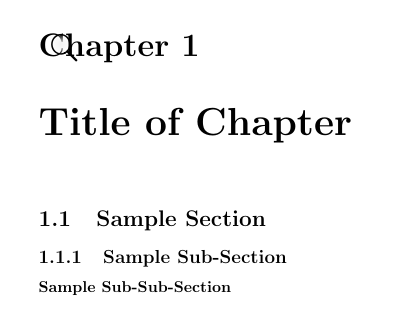
\includegraphics[width=0.5\linewidth]{sample-chapters-numbered.png}
		\end{figure}
		\column{0.5\textwidth}
		\textbf{Code:}
		{\tiny \begin{verbatim}
			\chapter*{Another Title}
			\section*{Sample Section}
			\subsection*{Sample Sub-Section}
			\subsubsection*{Sample Sub-Sub-Section}
		\end{verbatim}}
		\textbf{Output:}
		\begin{figure}
			\centering
			
\includegraphics[width=0.5\linewidth]{sample-chapters-unnumbered.png}
		\end{figure}
	\end{columns}
\end{frame}


\section{Equations and Formulas}

\begin{frame}[fragile]{Inline vs Block Math}
\textbf{Code:}
\begin{verbatim}
Inline math: $E = mc^2$

Block math:
\[
a^2 + b^2 = c^2
\]
\end{verbatim}

\vspace{0.5cm}

\textbf{Output:}

Inline math: $E = mc^2$

Block math:
\[
a^2 + b^2 = c^2
\]
\end{frame}

\begin{frame}[fragile]{Numbered Equations}
\textbf{Code:}
\begin{verbatim}
\begin{equation}
F = G \frac{m_1 m_2}{r^2}
\end{equation}
\end{verbatim}

\vspace{0.5cm}

\textbf{Output:}

\begin{equation}
F = G \frac{m_1 m_2}{r^2}
\end{equation}
\end{frame}

\begin{frame}[fragile]{Labeling and Referring Equations}
\textbf{Code:}
\begin{verbatim}
\begin{equation}
E = mc^2 \label{eq:einstein}
\end{equation}

As seen in equation~\ref{eq:einstein}, 
energy and mass are related.
\end{verbatim}

\vspace{0.5cm}

\textbf{Output:}

\begin{equation}
E = mc^2 \label{eq:einstein}
\end{equation}

As seen in equation~\ref{eq:einstein}, 
energy and mass are related.
\end{frame}

\begin{frame}{Online Tools to Make Latex Equations}

\begin{itemize}
    \item \textbf{Site 1} : \url{https://editor.codecogs.com/}
    \item \textbf{Site 2} : \url{https://latexeditor.lagrida.com/}
    \item \textbf{Site 3} : Use Overleaf Equation Generator or ChatGPT
\end{itemize}

\end{frame}

% Section: Tables
\section{Tables}

\begin{frame}[fragile]{Simple Table}
\textbf{Code:}
\begin{verbatim}
\begin{tabular}{c c}
A & B \\
C & D
\end{tabular}
\end{verbatim}

\vspace{0.5cm}

\textbf{Output:}

\begin{tabular}{c c}
A & B \\
C & D
\end{tabular}
\end{frame}

\begin{frame}[fragile]{Table with Borders}
\textbf{Code:}
\begin{verbatim}
\begin{tabular}{|c|c|}
\hline
Name & Score \\
\hline
Alice & 95 \\
Bob & 88 \\
\hline
\end{tabular}
\end{verbatim}

\vspace{0.5cm}

\textbf{Output:}

\begin{tabular}{|c|c|}
\hline
Name & Score \\
\hline
Alice & 95 \\
Bob & 88 \\
\hline
\end{tabular}
\end{frame}

\begin{frame}[fragile]{Table with Caption and Label}
\begin{columns}
\column{0.5\textwidth}
\textbf{Code:}
\begin{verbatim}
\begin{table}
\centering
\begin{tabular}{|c|c|}
\hline
Country & Capital \\
\hline
India & New Delhi \\
USA & Washington DC \\
\hline
\end{tabular}
\caption{List of Countries}
\label{tab:countries}
\end{table}

See Table~\ref{tab:countries} for details.
\end{verbatim}

\column{0.5\textwidth}

\textbf{Output:}

\begin{table}
\centering
\begin{tabular}{|c|c|}
\hline
Country & Capital \\
\hline
India & New Delhi \\
USA & Washington DC \\
\hline
\end{tabular}
\caption{List of Countries}
\label{tab:countries}
\end{table}
See Table~\ref{tab:countries} for details.
\end{columns}

\end{frame}

\begin{frame}[fragile]{Online Tools to Make Tables}

\begin{itemize}
    \item \textbf{Site 1} : \url{https://www.tablesgenerator.com/#}
    \item \textbf{Site 2} : \url{https://www.latex-tables.com/}
    \item \textbf{Site 3} : Use Overleaf Table Generator or ChatGPT
\end{itemize}

\end{frame}

% Section: Figures
\section{Figures}

\begin{frame}[fragile]{Including a Simple Image}
\textbf{Code:}
\begin{verbatim}

\includegraphics{rcoe-logo.png}
\end{verbatim}

\vspace{0.5cm}

\textbf{Output:}


\includegraphics{rcoe-logo.png}    

\end{frame}

\begin{frame}[fragile]{Resizing an Image}
\textbf{Code:}
\begin{verbatim}

\includegraphics[width=0.5\textwidth]{rcoe-logo.png}
\end{verbatim}

\vspace{0.5cm}

\textbf{Output:}


\includegraphics[width=0.5\textwidth]{rcoe-logo.png}
\end{frame}

\begin{frame}[fragile]{Image with Caption and Label}
\textbf{Code:}
\begin{verbatim}
\begin{figure}
\centering

\includegraphics[width=0.2\textwidth]{rcoe-logo.png}
\caption{Sample Figure}
\label{fig:sample}
\end{figure}

As shown in Figure~\ref{fig:sample}, 
this is an example image.
\end{verbatim}
\end{frame}

\begin{frame}{Image with Caption and Label: Output}
    
\textbf{Output:}

\begin{figure}
\centering

\includegraphics[width=0.2\textwidth]{rcoe-logo.png}
\caption{Sample Figure}
\label{fig:sample}
\end{figure}

As shown in Figure~\ref{fig:sample}, 
this is an example image.
\end{frame}

% Section: Citations and References
\section{Citations and References}

\begin{frame}[fragile]{Adding a Citation}
\textbf{Code:}
\begin{verbatim}
According to \cite{einstein}, 
energy and mass are related.
\end{verbatim}

\vspace{0.5cm}

\textbf{Output:}

According to \cite{einstein}, energy and mass are related.
\end{frame}

\begin{frame}[fragile]{Creating a .bib File}
\textbf{Code in refs.bib:}
\begin{verbatim}
@article{einstein,
  author  = {Albert Einstein},
  title   = {Does the Inertia of a Body Depend Upon Its Energy Content?},
  journal = {Annalen der Physik},
  year    = {1905},
}
\end{verbatim}

\textbf{Code in main.tex:}
\begin{verbatim}
\usepackage[backend=biber,style=ieee]{biblatex}  % preamble
\addbibresource{references.bib}

\printbibliography
\end{verbatim}
\end{frame}

\begin{frame}[fragile]{Output of References}
\textbf{Output:}

According to \cite{einstein}, energy and mass are related.

\vspace{0.5cm}

\textbf{References:}
\begin{thebibliography}{9}
\bibitem{einstein}
Albert Einstein.
\newblock Does the Inertia of a Body Depend Upon Its Energy Content?
\newblock {\em Annalen der Physik}, 1905.
\end{thebibliography}
\end{frame}


%----------------------------------------
% Hands-on Exercise: Resume
%----------------------------------------
\section{Exercise}

\begin{frame}[fragile]{Hands-on Exercise: Build Your Resume}
\textbf{Task:} Create a one-page resume using \LaTeX.

\bigskip
\textbf{Include the following:}
\begin{itemize}
    \item \textbf{Name} in large bold font
    \item \textbf{Tagline} (e.g., *"Student | Developer"*)
    \item \textbf{Photo} (insert with \verb|\includegraphics|)
    \item \textbf{Short Bio} (3–4 lines)
    \item \textbf{Education} (table or list with degree, year, institution)
    \item \textbf{Projects} (at least 2 with short description)
    \item \textbf{Skills} (list 5–6 skills)
\end{itemize}

\bigskip
\textbf{Bonus:} Use alignment, colors, and formatting to make it professional.
\end{frame}

\begin{frame}{Sample}
	\centering
    	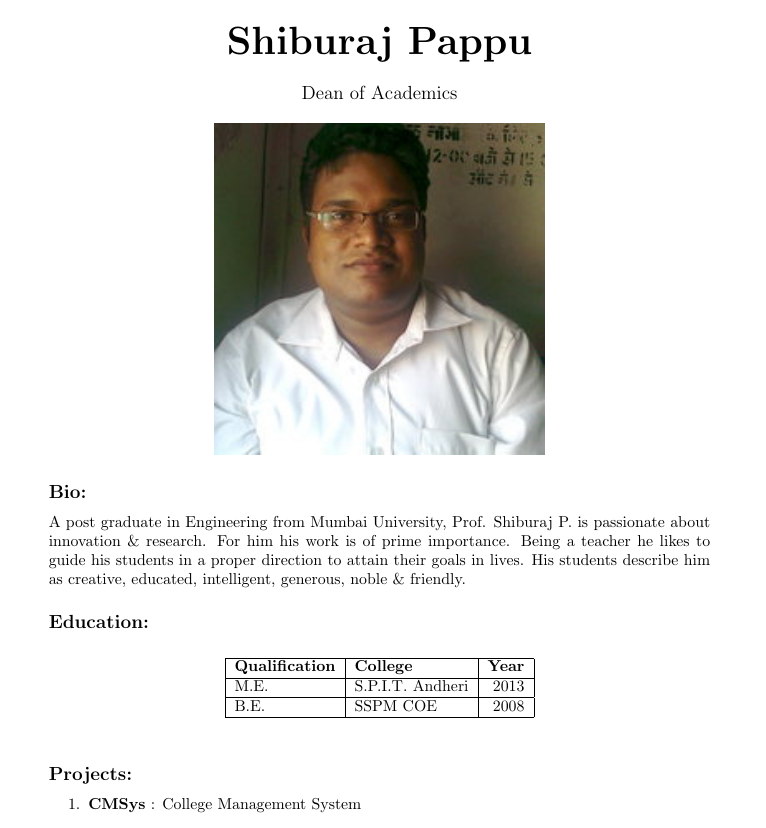
\includegraphics[width=0.5\textwidth]{excersice.png}
\end{frame}

% Questions Slide
\begin{frame}
	\centering
	{\Huge Thank You}
\end{frame}

\begin{frame}
  \centering
  {\Huge Questions?}
\end{frame}

\section{Report Templates}

\begin{frame}
  \begin{columns}
      \column{0.5\textwidth}
      \begin{figure}
          \centering
          
\includegraphics[width=0.5\linewidth]{synopsis.png}
      \end{figure}
      \centering
      \href{https://github.com/shiburaj/latex-synopsis-report}{\textbf{\textcolor{blue}{Synopsis Report Template}}}\\[1cm]
      {\small Use this template for Final year project synopsis report.}
      \column{0.5\textwidth}
      \begin{figure}
          \centering
          
\includegraphics[width=0.5\linewidth]{project.png}
      \end{figure}
      \centering
      \href{https://github.com/shiburaj/latex-project-report}{\textbf{\textcolor{blue}{Project Report Template}}}\\[1cm]
      {\small Use this template for Third/Final year project report.}
  \end{columns}
\end{frame}

\end{document}
